Se connecter sur ChromaCase avec Google vous permet de retrouver vos progrès et historique d’une session précédente, en utilisant votre compte Google.


Cliquez sur le bouton \textit{Continue With Google} (Voir Capture \ref{fig:signin-google}).

\begin{figure}[H]
	\begin{subfigure}[b]{0.7\textwidth}
		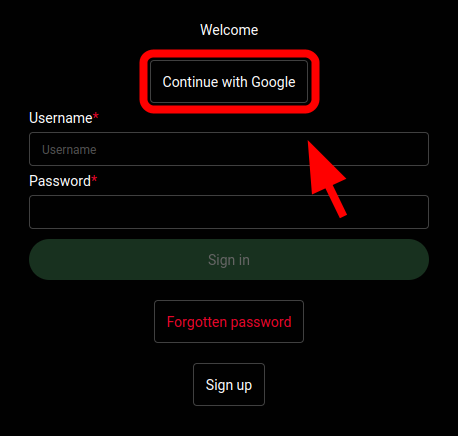
\includegraphics[width=\linewidth]{../\dir/guide/auth/signin-google.png}
		\caption{Version navigateur}
	\end{subfigure}
	\begin{subfigure}[b]{0.25\textwidth}
		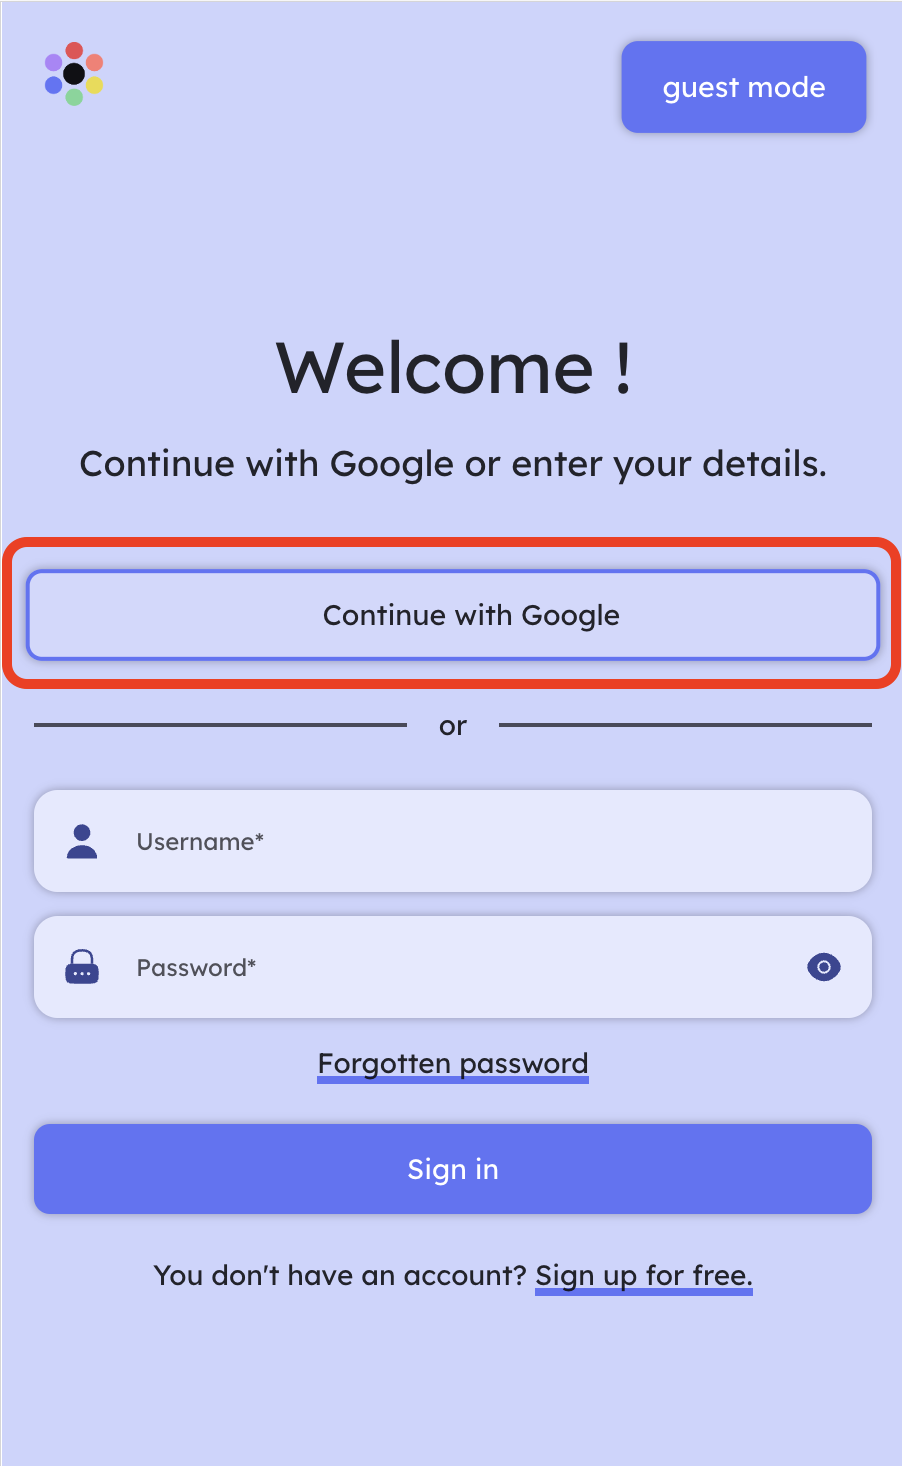
\includegraphics[width=\linewidth]{../\dir/guide/auth/signin-google-mobile.png}
		\caption{Version mobile}
	\end{subfigure}
	\caption{Se connecter avec Google}	
	\label{fig:signin-google}
\end{figure}

Vous serez redirigé vers un formulaire de connexion Google. Une fois rempli et validé, vous serez redirigé.e sur votre page personnelle.